% !TEX root = ../thesis.tex
% euclidic distance in norm notation
% @author Tobias Wulf
%

\section{Euklidischer Abstand in Normschreibweise}\label{sec:euklidischer-abstand}


Um adäquate Bezüge bzw. Abstände zwischen einzelnen Messwerten herzustellen ist ein Wechsel der Betrachtungsweise notwendig. Es erleichtert die Handhabung der Problemstellung Vektorbeträge als normierte Längen und Distanzen zu sehen. Betrachtet man die vektoriellen Zusammenhänge, der klassischen Anwendung aus \autoref{sec:kreisdarstellung-anwendung}, in Normschreibweise. Ergibt sich der Radius $r$ für eine Winkelstellung $\mathbf{A}\mapsto\alpha_1$ nach \autoref{eq:rinnorm}. Die einzelnen Vektorelemente sind entsprechend der Vektor-2-Norm \cite{vandeGeijn2014} zum Radius $r$ normiert.


\begin{equation}\label{eq:rinnorm}
r = |\mathbf{A}| =\sqrt{a_x^2 + a_y^2} = \sqrt{\sum_{i=1}^{n}|A_i|^2} = \|\mathbf{A}\|_2
\end{equation}


Es ist weithin von einer idealen Ausrichtung von Sensor und Gebermagnet wie in \autoref{fig:klassischeranwendungsfall} auszugehen. Somit bleibt der Kreisbahn Radius $r$ für eine zweite Winkelstellung mit $\mathbf{B}\mapsto\alpha_2$ konstant.


\begin{equation}
r = \|\mathbf{A}\|_2 = \|\mathbf{B}\|_2 = konst.
\end{equation}


Der direkte Abstand zwischen den beiden Winkelstellung $\mathbf{A}\mapsto\alpha_1$ und $\mathbf{B}\mapsto\alpha_2$ lässt sich geometrisch über den Satz des Pythagoras ermitteln. Dafür werden Abstandquadrate aus den Einzeldifferenzen der vektoriellen $X$-/ $Y$-Anteile gebildet. Das Resultierende Abstandsquadrat bildet mit seiner Kantenlänge dann den Winkelabstand zwischen beiden Winkelstellungen. \autoref{fig:kreisdarstellungwinkelabstand} veranschaulicht das Vorgehen.


\begin{align}\label{eq:deinnorm}
d_E\langle\mathbf{A},\mathbf{B}\rangle &= \sqrt{(a_x - b_x)^2 + (a_y - b_y)^2} \nonumber \\
&= \sqrt{\sum_{i=1}^{n}(A_i - B_i)^2} = \|\mathbf{A} - \mathbf{B}\|_2
\end{align}


\clearpage


Die Überführung in Normschreibweise des Abstandes ergibt nach \autoref{eq:deinnorm} eine Vektor-2-Differenznorm und ist allgemein als euklidischer Abstand bekannt. Analog dazu bildet sich das Quadrat nach \autoref{eq:de2innorm}.


\begin{equation}\label{eq:de2innorm}
d_E^2\langle\mathbf{A},\mathbf{B}\rangle = (a_x - b_x)^2 + (a_y - b_y)^2 = \|\mathbf{A} - \mathbf{B}\|_2^2
\end{equation}

\vspace{5mm}
\begin{figure}[bph]
	\centering
	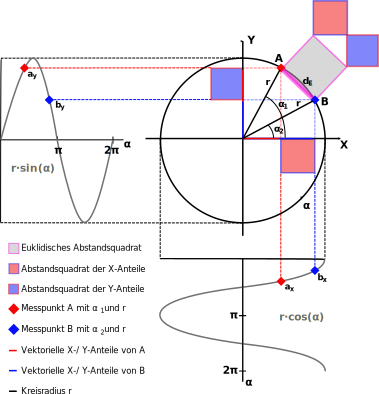
\includegraphics[width=0.7\linewidth]{chapters/images/2-Grundlagen/Kreisdarstellung_Winkelabstand}
	\caption[Allg. Kreisdarstellung des euklidischen Winkelabstands]{Allg. Kreisdarstellung des euklidischen 
		Winkelabstands. Die Kreisdarstellung zeigt den euklidischen Winkelabstand zweier Winkelmesspunkte $\mathbf{A}$ 
		und $\mathbf{B}$ mit gleichen Kreisradius $r$. Der euklidische Abstand, bzw. das Abstandsquadrat, zwischen den 
		Winkelposition $\mathbf{A}$ und $\mathbf{B}$ ist zerlegt in Abstandsquadratanteile. Die Abstandquadratanteile 
		ergeben sich aus der vektoriellen Zusammensetzung in $X$-/ $Y$-Anteile für die einzelnen Messpunkte 
		$\mathbf{A}$ und $\mathbf{B}$.}
	\label{fig:kreisdarstellungwinkelabstand}
\end{figure}


\clearpage


Für Vektor-2-Normen muss die Dreiecksungleichung aus \autoref{eq:v2ungleichung} \cite{Plum2012}\cite{vandeGeijn2014} gelten. Über die Ungleichung lassen sich Einzelnormen approximiert im Vergleich zu Differenznormen zwischen zwei Punkten $\mathbf{A}$ und $\mathbf{B}$ darstellen. Dieser Ansatz kann genutzt werden wenn die Bahnradius $r$ nicht mehr konstant ist und somit $\|\mathbf{A}\|_2 \ne \|\mathbf{B}\|_2$ ist. Der Ansatz begünstigt die Projektion von orthogonalen Systemen in höheren Normraum \cite{Plum2012} und stellt somit die Grundlage für eine Adaptierung auf ein Sensor-Array dar.


\begin{gather}\label{eq:v2ungleichung}
\big| \|\mathbf{A}\|_2 - \|\mathbf{B}\|_2 \big| \le
	\|\mathbf{A} \pm \mathbf{B}\|_2 \le \big| \|\mathbf{A}\|_2 + \|\mathbf{B}\|_2 \big| \nonumber \\
\Updownarrow \\
\big(\|\mathbf{A}\|_2 - \|\mathbf{B}\|_2\big)^2 \le \|\mathbf{A} \pm \mathbf{B}\|_2^2 \le
	\big(\|\mathbf{A}\|_2 + \|\mathbf{B}\|_2\big)^2 \nonumber
\end{gather}

